\documentclass[12pt]{article}

\usepackage[margin=1in]{geometry}
\usepackage{fancyhdr}
\usepackage{amsmath, amsfonts, amsthm, amssymb, mathtools}  % Some math symbols
\usepackage{color}
% \usepackage{sectsty}
\usepackage{tcolorbox}
\usepackage{amsfonts}
\usepackage{titletoc}
\usepackage{caption}
\usepackage[normalem]{ulem}
\usepackage{graphicx}


\usepackage{hyperref}
\hypersetup{
    colorlinks,
    citecolor=black,
    filecolor=black,
    linkcolor=black,
    urlcolor=black
}


\titlecontents{section}[0em]
{\smallskip}
{\thecontentslabel\enspace}
{\hspace*{-5.3em}}
{\hfill\contentspage}



%%%%%%%%%%%% SETUP %%%%%%%%%%%%

% name of the class
\newcommand{\classname}{CSE 371}
% name of the assignment
\newcommand{\assignmentname}{HW5}
% collaborators on assignment
\newcommand{\collaborators}{Cameron Jennings (ID: 2029631), Donovan Clay (ID: 2276005)}
\newcommand{\listcollaborators}{Collaborators: \collaborators}

\pagestyle{fancy}
\fancyhf{}
\setlength{\headheight}{13.59999pt}
\rhead{\thepage}
\lhead{\hyperref[beginning]{\classname \hspace{1em} \assignmentname}}

\usepackage{titlesec}
\titleformat{\subsection}{\normalfont\fontsize{12}{15}\bfseries}{\thesubsection}{1em}{}

\titleformat{\section}[block]
{\filcenter\large
\addtolength{\titlewidth}{2pc}%
\titleline*[c]{}%
\addvspace{6pt}%
}
{\thesection}{1em}{}
\titlespacing{\section}
{5pc}{*2}{*2}[5pc]


% \definecolor{WordSectionBlue}{RGB}{30, 90, 147}
% \allsectionsfont{\color{WordSectionBlue}}

%%%%%%%%%%%% FILE SPECIFIC IMPORTS %%%%%%%%%%%%

\usepackage{ragged2e}
\usepackage{tikz}

%%%%%%%%%%%%%%%%%%%%%%%%%%%%%%%%%%%%%%%%%%%%%%%

\renewcommand*{\thesection}{Question \arabic{section}.}
\renewcommand{\thesubsection}{(\alph{subsection})}

%%%%%%%%%%%% ENVIRONMENTS %%%%%%%%%%%%

\newenvironment{explanation}{\begin{tcolorbox}[colback=blue!2!white,colframe=blue!20!white]}{\end{tcolorbox}}

\newenvironment{subquestion}[1]{\subsection{#1}
\begin{tcolorbox}[colback=blue!2!white,colframe=blue!20!white]}{\end{tcolorbox}}

\newenvironment{sssq}[3]{\textbf{\thesubsubsection.\sssqARG{#1}} \hspace{0.5cm}
\begin{minipage}[t][\sssqARG{#2}][t]{14cm}
    \textbf{\sssqARG{#3}}
\end{minipage}
\begin{explanation}
}{\end{explanation}}

%%%%%%%%%%%% MY MACROS %%%%%%%%%%%%

\newcommand{\prob}{\mathbb{P}}
\newcommand{\expect}{\mathbb{E}}
\newcommand*\sssqARG{}
\newcommand{\bayes}{\textbf{Bayes' Theorem}}
\newcommand{\ltp}{\textbf{Law of Total Probability}}
\newcommand{\var}{\text{Var}}
\newcommand{\unif}{\sim \text{Unif}}
\newcommand{\expo}{\sim \text{Exponential}}
\newcommand{\caseif}{\text{if }}
\newcommand{\nlog}{\text{ln}}
\newcommand{\dat}{\text{DAT}}
\newcommand{\drt}{\text{DRT}}
\newcommand{\clk}{\text{clk}}
\newcommand{\ns}{\text{ns}}


%%%%%%%%%%%%%%%%%%%%%%%%%%%%%%%%%%%%%%
\begin{document}

    \setcounter{tocdepth}{1}
    \begin{center}\label{beginning}
        \tableofcontents 
    \end{center}

    \begin{center}
        \listcollaborators
    \end{center}

    % fix section heading font
    \titleformat{\section}{\normalfont\fontsize{17.28}{15}\bfseries\raggedright}{\thesection}{1em}{}
    \newpage
    \AddToHook{cmd/section/before}{\clearpage}

    % Question 1
    \section{}
        \begin{explanation}
            \begin{align*}
                \text{hold slack} &= \dat_h - \drt_h \\
                &= \text{min data path} - \text{max clock path} \\
                &= (T_{\clk 1} + T_{\text{CO}} + T_{\text{data min}}) - (T_{\clk 2} + T_{\text{hold}}) \\
                &= 6 \text{ns} - 3.5 \text{ns} \\
                &= 2.5 \text{ns}
            \end{align*}

            The hold slack meets timing requirements.

            \begin{align*}
                \text{setup slack} &= \drt_{\text{su}} - \dat_\text{su} \\
                &= \text{min clock path} - \text{max data path} \\
                &= (T + T_{\clk 2} - t_{\text{su}}) - (T_{\text{\clk 1}} + T_{\text{CO}} + T_{\text{data max}}) \\
                &= (6.67\ns + 2\ns - 2\ns) - (1\ns + 2\ns + 5 \ns) \\
                &= -1.33 \ns
            \end{align*}

            \underline{The setup slack does not meet the timing requirements because it is negative.}
        \end{explanation}
    
    \section{}
        \begin{explanation}
            The max data path is In $\rightarrow$ AND $\rightarrow$ NOR $\rightarrow$ reg1.
            \begin{align*}
                \text{setup slack} &= \drt_{\text{su}} - \dat_\text{su} \\
                &= \text{min clock path} - \text{max data path} \\
                &= (T_\text{period} + T_{\clk 1, \text{min}} - t_{\text{su}}) - (T_{\text{in, max}} + T_{\text{AND, max}} + T_{\text{NOR, max}}) \\
                &= (100 \ns + 4 \ns - 10 \ns) - (17 \ns + 40 \ns + 30\ns) \\
                &= 94 \ns - 87 \ns \\
                &= 7 \ns
            \end{align*}

            The min clock path is reg1 $\rightarrow$ AND $\rightarrow$ reg2.
            \begin{align*}
                \text{hold slack} &= \dat_h - \drt_h \\
                &= \text{min data path} - \text{max clock path} \\
                &= (T_{\clk 1, \text{min}} + T_{\text{CO, min}} + T_{\text{AND, min}}) - (T_{\text{launch}} + T_{\clk 2, \text{max}} + T_{\text{hold}}) \\
                &= (4\ns + 8\ns + 35\ns) - (0 \ns + 3 \ns + 5\ns) \\
                &= 47 \ns - 8\ns \\
                &= 39 \ns
            \end{align*}
        \end{explanation}

    \section{}
        \begin{subquestion}{Draw the DFG}
            \begin{center}
                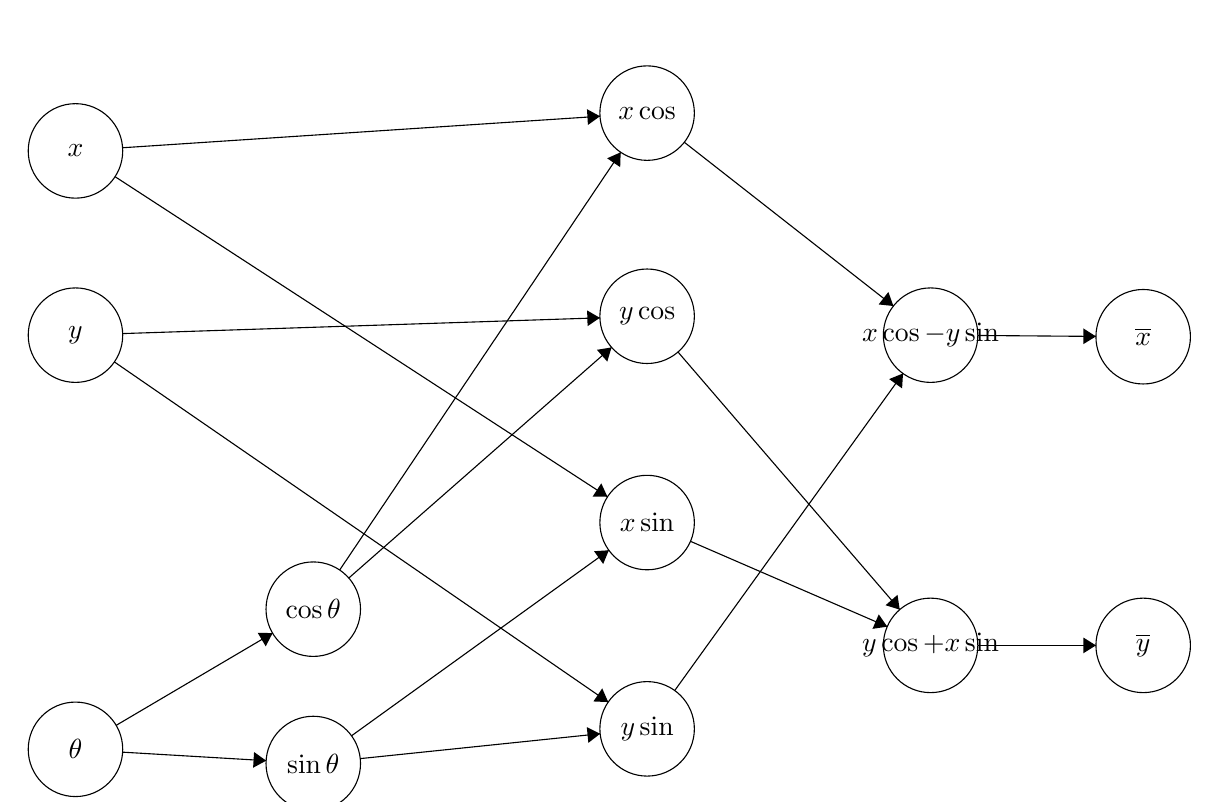
\begin{tikzpicture}[scale=0.2]
                \tikzstyle{every node}+=[inner sep=0pt]
                \draw [black] (9.2,-14.7) circle (3);
                \draw (9.2,-14.7) node {$x$};
                \draw [black] (9.2,-26.4) circle (3);
                \draw (9.2,-26.4) node {$y$};
                \draw [black] (9.2,-52.7) circle (3);
                \draw (9.2,-52.7) node {$\theta$};
                \draw [black] (24.3,-43.8) circle (3);
                \draw (24.3,-43.8) node {$\cos\theta$};
                \draw [black] (45.5,-12.3) circle (3);
                \draw (45.5,-12.3) node {$x\cos$};
                \draw [black] (45.5,-25.2) circle (3);
                \draw (45.5,-25.2) node {$y\cos$};
                \draw [black] (45.5,-38.3) circle (3);
                \draw (45.5,-38.3) node {$x\sin$};
                \draw [black] (24.3,-53.6) circle (3);
                \draw (24.3,-53.6) node {$\sin\theta$};
                \draw [black] (45.5,-51.4) circle (3);
                \draw (45.5,-51.4) node {$y\sin$};
                \draw [black] (63.5,-26.4) circle (3);
                \draw (63.5,-26.4) node {$x\cos-y\sin$};
                \draw [black] (63.5,-46.1) circle (3);
                \draw (63.5,-46.1) node {$y\cos+x\sin$};
                \draw [black] (77,-26.5) circle (3);
                \draw (77,-26.5) node {$\overline{x}$};
                \draw [black] (77,-46.1) circle (3);
                \draw (77,-46.1) node {$\overline{y}$};
                \draw [black] (11.78,-51.18) -- (21.72,-45.32);
                \fill [black] (21.72,-45.32) -- (20.77,-45.3) -- (21.28,-46.16);
                \draw [black] (12.19,-14.5) -- (42.51,-12.5);
                \fill [black] (42.51,-12.5) -- (41.68,-12.05) -- (41.74,-13.05);
                \draw [black] (25.98,-41.31) -- (43.82,-14.79);
                \fill [black] (43.82,-14.79) -- (42.96,-15.17) -- (43.79,-15.73);
                \draw [black] (12.2,-26.3) -- (42.5,-25.3);
                \fill [black] (42.5,-25.3) -- (41.69,-24.83) -- (41.72,-25.83);
                \draw [black] (26.56,-41.82) -- (43.24,-27.18);
                \fill [black] (43.24,-27.18) -- (42.31,-27.33) -- (42.97,-28.08);
                \draw [black] (12.19,-52.88) -- (21.31,-53.42);
                \fill [black] (21.31,-53.42) -- (20.54,-52.87) -- (20.48,-53.87);
                \draw [black] (26.73,-51.84) -- (43.07,-40.06);
                \fill [black] (43.07,-40.06) -- (42.13,-40.12) -- (42.71,-40.93);
                \draw [black] (11.72,-16.34) -- (42.98,-36.66);
                \fill [black] (42.98,-36.66) -- (42.59,-35.81) -- (42.04,-36.65);
                \draw [black] (27.28,-53.29) -- (42.52,-51.71);
                \fill [black] (42.52,-51.71) -- (41.67,-51.29) -- (41.77,-52.29);
                \draw [black] (11.67,-28.1) -- (43.03,-49.7);
                \fill [black] (43.03,-49.7) -- (42.65,-48.83) -- (42.09,-49.66);
                \draw [black] (47.25,-48.97) -- (61.75,-28.83);
                \fill [black] (61.75,-28.83) -- (60.87,-29.19) -- (61.69,-29.78);
                \draw [black] (47.86,-14.15) -- (61.14,-24.55);
                \fill [black] (61.14,-24.55) -- (60.82,-23.66) -- (60.2,-24.45);
                \draw [black] (48.25,-39.49) -- (60.75,-44.91);
                \fill [black] (60.75,-44.91) -- (60.21,-44.13) -- (59.81,-45.05);
                \draw [black] (47.46,-27.47) -- (61.54,-43.83);
                \fill [black] (61.54,-43.83) -- (61.4,-42.89) -- (60.64,-43.55);
                \draw [black] (66.5,-46.1) -- (74,-46.1);
                \fill [black] (74,-46.1) -- (73.2,-45.6) -- (73.2,-46.6);
                \draw [black] (66.5,-26.42) -- (74,-26.48);
                \fill [black] (74,-26.48) -- (73.2,-25.97) -- (73.2,-26.97);
                \end{tikzpicture}
            \end{center}
        \end{subquestion}

        \begin{subquestion}{Cuts}
            \begin{description}
                \item \textbf{1 stage cut} \\
                    \begin{center}
                        \includegraphics[scale = 0.5]{Images/1 stage cut.png}
                    \end{center}
                    The clock period for this pipelined circuit is: $$\text{max}(10\ns + 100\ns, 10\ns + 60\ns + 30\ns) = 110\ns$$.
                \item \textbf{2 stage cut} \\
                    \begin{center}
                        \includegraphics[scale = 0.5]{Images/2 stage cut.png}
                    \end{center}
                    The clock period for this pipelined circuit is: $$\text{max}(10\ns + 100\ns, 10\ns + 60\ns, 10\ns + 30\ns) = 110\ns$$.
            \end{description}
        \end{subquestion}

        \begin{subquestion}{}
            \begin{description}
                \item \textbf{2-stage} \\
                    \begin{align*}
                        \text{latency} &= \text{\# of stages} \cdot T_{\text{period}} + T_{\text{CO}} \\
                        &= 2 \cdot 110\ns + 10 \ns \\
                        &= 220 \ns + 10 \ns \\
                        &= 230 \ns
                    \end{align*}
                \item \textbf{3-stage} \\
                    \begin{align*}
                        \text{latency} &= \text{\# of stages} \cdot T_{\text{period}} + T_{\text{CO}} \\
                        &= 3 \cdot 110\ns + 10 \ns \\
                        &= 330 \ns + 10 \ns \\
                        &= 340 \ns
                    \end{align*}
            \end{description}
        \end{subquestion}

    \section{}
        \begin{subquestion}{What element adds the most delay?}
            The datapath adds the most delay with 16.138ns. The DRT is 15.989ns. DAT is 20.248 ns. Using setup slack equation, DRT - DAT, this would give us -4.259ns. To ensure setup meets timing requirements, we should add at least 4.259ns.
        \end{subquestion}

        \begin{subquestion}{Does the same element add the most delay for hold slack? Why does this make sense?}
            No. The longest timing element in delay slack is the clock delay. This makes makes sense because it's the longest clock path which determines the hold slack.
        \end{subquestion}

        \begin{subquestion}{What is the fastest frequency you can set the clock to for this to pass setup timing?}
            The new DAT is 16.759ns. Therefore that's the period we need for our clock. The frequency would be $\frac{1}{16.759\ns}$ which gives $5.96 \times 10^7\text{Hz}$.
        \end{subquestion}
        
        \begin{subquestion}{SETUP: Which of the options had the most setup slack?}
            Fast/0C
        \end{subquestion}

        \begin{subquestion}{SETUP: How does increasing voltage speed change the speed of a circuit?}
            Increasing voltage increases speed.
        \end{subquestion}

        \begin{subquestion}{SETUP: How does increasing temperature change the speed of a circuit?}
            Increasing temperature slows down the circuit
        \end{subquestion}

        \begin{subquestion}{HOLD: Which of the options had the most hold slack?}
            Fast/0C
        \end{subquestion}

        \begin{subquestion}{HOLD: How does increasing voltage speed change the speed of a circuit?}
            Increasing voltage increases speed.
        \end{subquestion}

        \begin{subquestion}{HOLD: How does increasing temperature change the speed of a circuit?}
            Increasing temperature slows down the circuit
        \end{subquestion}

    \section{Experience Report}
        We found this homework to be moderate. Question 3 had some tricky parts where we almost forgot to add the last $T_{\text{CO}}$. Question 4 took a while.
        \begin{description}
            \item[Question 1:] 30 minutes
            \item[Question 2:] 30 minutes
            \item[Question 3:] 30 minutes
            \item[Question 4:] 1 hour.
        \end{description}        
\end{document}
